\documentclass[a4paper,twoside,master.tex]{subfiles}
\begin{document}
\lecture{18}{Mon Sep 30 2019}{Interference}

\section{Interference}%
\label{sec:interference}

Imagine we are throwing baseballs at a wall with two slits (yes, we're just rehashing the double-slit experiment). With baseballs, we notice two things. The baseballs are caught one at a time (they are discrete events), and there is a smooth distribution for where the balls land when they reach the ``catcher''. If we take the distributions for balls which go through each slit, the total distribution is equal to the sum of both distributions ($P_{12} = P_1 + P_2 $). The conditional probability $P_1 $ is the same whether or not slit $2$ is open or closed.

Now let's imagine the same scenario with water waves. We can imagine these waves passing through slits in the wall, and the wave crests coming out of both slits will interfere with each other. If one slit is open and the other closed, we would see some sort of unimodal distribution, but if both are open, we see that $I_{12} \neq I_1 + I_2$ ($I$ for ``intensity''). The arrival of the wave is continuous (no discrete events for detection). With the waves, there is no analog of conditional probability. Manifestly, if both slits are open, the wave goes through both slits simultaneously, so the conditional probability is meaningless here. We could also put a phase-shifter behind one or both of the slits (something that slows the wave temporarily). If we put it behind one, we would see the pattern shifted one way or the other, and if we put it behind both, nothing would change. The position of the largest peak depends on the phase difference between the waves leaving both slits.

What would we see if we did this experiment with electrons? Every item of this list has been experimentally verified:
\begin{itemize}
    \item[1.] Electrons arrive as individual events.
    \item[2.] Probabilities $P_{12} \neq P_1 + P_2$. We see an interference pattern similar to the water waves example.
    \item[3.] We can detect if a particle goes through the slit by scattering short wavelength photons. However, when we do this, $P_{12} = P_1 + P_2$.
    \item[4.] We can detect if the particle passes through either slit with long wavelength photons (although you wouldn't be able to see which slit the particle goes through. Under this condition, the interference pattern is preserved.
        \item[5.] If we ``weakly'' detect the slit (short wavelength, but low intensity, many electrons are not detected at all), we see a partial interference pattern.
\end{itemize}

Now we can start asking questions. Does the electron go through both slits? The final events are localized, unlike water waves. We detect singular events with definite position on the screen. If we say that the electron is localized, it can't go through both slits. However, there is an interference pattern, which would seem to require that the electron did go through both holes. However, when we use intense, short wavelength light to see which hole the electron passes through, we clearly only detect it going through one or the other.

\subsection{Mach-Zehnder Interferometer}
\begin{figure}[h]
    \centering
    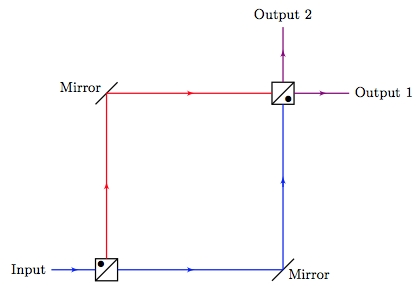
\includegraphics{mach_zehnder_interferometer}
    \caption{A Mach-Zehnder Interferometer}
    \label{fig:mz_inter}
\end{figure}

We will label the following paths. The input in the bottom right of the diagram will be path $a$, the downward path from here will be $b$, the upward path will go from $1c$ between the beam splitter and mirror, $2c$ at the mirror, $3c$ between the mirror and the second beam splitter, and then $4f$ after the second beam splitter. The same will follow for the other branch using the labels $d$ and $e$. Our time evolution operator is our shift operator $(T=S)$. Here
\begin{equation}
    S\ket{mz} = \ket{(m+1)z}
\end{equation}
\begin{align}
    S\ket{0a} &= \frac{1}{\sqrt{2}}(\ket{1c}+\ket{1d})\\
    S\ket{0b} &= \frac{1}{\sqrt{2}} (-\ket{1c}+\ket{1d})\\
    S\ket{3c} &= \frac{1}{\sqrt{2}} (\ket{4e} + \ket{4f} )\\
    S\ket{3d} &= \frac{1}{\sqrt{2}} (-\ket{4e}+\ket{4f})
\end{align}
We see that, for the two paths,
\begin{align}
    \ket{m \overline{a}} &\equiv \frac{1}{\sqrt{2}} (\ket{mc} + \ket{md})\\
    \ket{m \overline{b}} &\equiv \frac{1}{\sqrt{2}} (-\ket{mc} + \ket{md})
\end{align}
For example
\begin{equation}
    T\ket{3 \overline{a}} = \frac{1}{\sqrt{2}} (\ket{4c} + \ket{4d})
\end{equation}
Imagine we now have phase shifters $\phi_{c,d}$ between points $2$ and $3$ in the respective channels. We say the phase shifters operate as:
\begin{equation}
    S\ket{2x} = e^{\imath\phi_x}\ket{3x}
\end{equation}
for channel $x$.
\begin{equation}
    \ket{0a} \to \ket{1 \overline{a}} \to \ket{2 \overline{a}} \to \frac{1}{\sqrt{2}} (e^{\imath\phi_c} \ket{3c} + e^{\imath\phi_d} \ket{3d}) \to \frac{1}{2} (e^{\imath\phi_c} (\ket{4e} + \ket{4f}) + e^{\imath\phi_d} (-\ket{4e} + \ket{4f})
\end{equation}
Let's write down the nonzero chainkets for this scenario:
\begin{equation}
    Y^e = [0a]_0 \odot [4e]_4
\end{equation}
\begin{equation}
    Y^f = [0a]_0 \odot [4f]_4
\end{equation}
since
\begin{equation}
    \ket{Y^e} = [4e]T^4\ket{0a} = \frac{1}{2} (e^{\imath\phi_c} - e^{\imath\phi_d}\ket{4e}
\end{equation}
and
\begin{equation}
    \ket{Y^f} = [4f]T^4\ket{0a} = \frac{1}{2} (e^{\imath\phi_c} + e^{\imath\phi_d}\ket{4f}
\end{equation}
We can also work out
\begin{equation}
    \Pr(Y^e) = \frac{1}{4} \norm{e^{\imath\phi_c} - e^{\imath\phi_d}}^2 = \sin[2](\Delta/2)
\end{equation}
and
\begin{equation}
    \Pr(Y^f) \cos[2](\Delta/2)
\end{equation}
where
\begin{equation}
    \Delta = \phi_c - \phi_d \in [0, 2\pi]
\end{equation}
On Wednesday, we will start asking the question of which path the photon took if we know where it exited. This will be equivalent to asking which slit an electron goes through the double slit experiment when it creates the interference pattern.

\end{document}
